%% SOA_Baluta_Sandu_rezumat.tex
%% by Gabriel Sandu and Daniel Baluta
%% Paper based on bare_conf.tex template from IEEE Transaction class

%% bare_conf.tex
%% V1.3
%% 2007/01/11
%% by Michael Shell
%% See:
%% http://www.michaelshell.org/
%% for current contact information.
%%
%% This is a skeleton file demonstrating the use of IEEEtran.cls
%% (requires IEEEtran.cls version 1.7 or later) with an IEEE conference paper.
%%
%% Support sites:
%% http://www.michaelshell.org/tex/ieeetran/
%% http://www.ctan.org/tex-archive/macros/latex/contrib/IEEEtran/
%% and
%% http://www.ieee.org/

%%*************************************************************************
%% Legal Notice:
%% This code is offered as-is without any warranty either expressed or
%% implied; without even the implied warranty of MERCHANTABILITY or
%% FITNESS FOR A PARTICULAR PURPOSE! 
%% User assumes all risk.
%% In no event shall IEEE or any contributor to this code be liable for
%% any damages or losses, including, but not limited to, incidental,
%% consequential, or any other damages, resulting from the use or misuse
%% of any information contained here.
%%
%% All comments are the opinions of their respective authors and are not
%% necessarily endorsed by the IEEE.
%%
%% This work is distributed under the LaTeX Project Public License (LPPL)
%% ( http://www.latex-project.org/ ) version 1.3, and may be freely used,
%% distributed and modified. A copy of the LPPL, version 1.3, is included
%% in the base LaTeX documentation of all distributions of LaTeX released
%% 2003/12/01 or later.
%% Retain all contribution notices and credits.
%% ** Modified files should be clearly indicated as such, including  **
%% ** renaming them and changing author support contact information. **
%%
%% File  of work: IEEEtran.cls, IEEEtran_HOWTO.pdf, bare_adv.tex,
%%                    bare_conf.tex, bare_jrnl.tex, bare_jrnl_compsoc.tex
%%*************************************************************************

% *** Authors should verify (and, if needed, correct) their LaTeX system  ***
% *** with the testflow diagnostic prior to trusting their LaTeX platform ***
% *** with production work. IEEE's font choices can trigger bugs that do  ***
% *** not appear when using other class files.                            ***
% The testflow support page is at:
% http://www.michaelshell.org/tex/testflow/



% Note that the a4paper option is mainly intended so that authors in
% countries using A4 can easily print to A4 and see how their papers will
% look in print - the typesetting of the document will not typically be
% affected with changes in paper size (but the bottom and side margins will).
% Use the testflow package mentioned above to verify correct handling of
% both paper sizes by the user's LaTeX system.
%
% Also note that the "draftcls" or "draftclsnofoot", not "draft", option
% should be used if it is desired that the figures are to be displayed in
% draft mode.
%
\documentclass[conference]{IEEEtran}
% Add the compsoc option for Computer Society conferences.
%
% If IEEEtran.cls has not been installed into the LaTeX system files,
% manually specify the path to it like:
% \documentclass[conference]{../sty/IEEEtran}





% Some very useful LaTeX packages include:
% (uncomment the ones you want to load)


% *** MISC UTILITY PACKAGES ***
%
%\usepackage{ifpdf}
% Heiko Oberdiek's ifpdf.sty is very useful if you need conditional
% compilation based on whether the output is pdf or dvi.
% usage:
% \ifpdf
%   % pdf code
% \else
%   % dvi code
% \fi
% The latest version of ifpdf.sty can be obtained from:
% http://www.ctan.org/tex-archive/macros/latex/contrib/oberdiek/
% Also, note that IEEEtran.cls V1.7 and later provides a builtin
% \ifCLASSINFOpdf conditional that works the same way.
% When switching from latex to pdflatex and vice-versa, the compiler may
% have to be run twice to clear warning/error messages.






% *** CITATION PACKAGES ***
%
%\usepackage{cite}
% cite.sty was written by Donald Arseneau
% V1.6 and later of IEEEtran pre-defines the format of the cite.sty package
% \cite{} output to follow that of IEEE. Loading the cite package will
% result in citation numbers being automatically sorted and properly
% "compressed/ranged". e.g., [1], [9], [2], [7], [5], [6] without using
% cite.sty will become [1], [2], [5]--[7], [9] using cite.sty. cite.sty's
% \cite will automatically add leading space, if needed. Use cite.sty's
% noadjust option (cite.sty V3.8 and later) if you want to turn this off.
% cite.sty is already installed on most LaTeX systems. Be sure and use
% version 4.0 (2003-05-27) and later if using hyperref.sty. cite.sty does
% not currently provide for hyperlinked citations.
% The latest version can be obtained at:
% http://www.ctan.org/tex-archive/macros/latex/contrib/cite/
% The documentation is contained in the cite.sty file itself.






% *** GRAPHICS RELATED PACKAGES ***
%
\ifCLASSINFOpdf
\usepackage[pdftex]{graphicx}
  % declare the path(s) where your graphic files are
  % \graphicspath{{../pdf/}{../jpeg/}}
  % and their extensions so you won't have to specify these with
  % every instance of \includegraphics
\DeclareGraphicsExtensions{.pdf,.jpeg,.png}
\else
  % or other class option (dvipsone, dvipdf, if not using dvips). graphicx
  % will default to the driver specified in the system graphics.cfg if no
  % driver is specified.
  % \usepackage[dvips]{graphicx}
  % declare the path(s) where your graphic files are
  % \graphicspath{{../eps/}}
  % and their extensions so you won't have to specify these with
  % every instance of \includegraphics
  % \DeclareGraphicsExtensions{.eps}
\fi
% graphicx was written by David Carlisle and Sebastian Rahtz. It is
% required if you want graphics, photos, etc. graphicx.sty is already
% installed on most LaTeX systems. The latest version and documentation can
% be obtained at: 
% http://www.ctan.org/tex-archive/macros/latex/required/graphics/
% Another good source of documentation is "Using Imported Graphics in
% LaTeX2e" by Keith Reckdahl which can be found as epslatex.ps or
% epslatex.pdf at: http://www.ctan.org/tex-archive/info/
%
% latex, and pdflatex in dvi mode, support graphics in encapsulated
% postscript (.eps) format. pdflatex in pdf mode supports graphics
% in .pdf, .jpeg, .png and .mps (metapost) formats. Users should ensure
% that all non-photo figures use a vector format (.eps, .pdf, .mps) and
% not a bitmapped formats (.jpeg, .png). IEEE frowns on bitmapped formats
% which can result in "jaggedy"/blurry rendering of lines and letters as
% well as large increases in file sizes.
%
% You can find documentation about the pdfTeX application at:
% http://www.tug.org/applications/pdftex





% *** MATH PACKAGES ***
%
%\usepackage[cmex10]{amsmath}
% A popular package from the American Mathematical Society that provides
% many useful and powerful commands for dealing with mathematics. If using
% it, be sure to load this package with the cmex10 option to ensure that
% only type 1 fonts will utilized at all point sizes. Without this option,
% it is possible that some math symbols, particularly those within
% footnotes, will be rendered in bitmap form which will result in a
% document that can not be IEEE Xplore compliant!
%
% Also, note that the amsmath package sets \interdisplaylinepenalty to 10000
% thus preventing page breaks from occurring within multiline equations. Use:
%\interdisplaylinepenalty=2500
% after loading amsmath to restore such page breaks as IEEEtran.cls normally
% does. amsmath.sty is already installed on most LaTeX systems. The latest
% version and documentation can be obtained at:
% http://www.ctan.org/tex-archive/macros/latex/required/amslatex/math/





% *** SPECIALIZED LIST PACKAGES ***
%
%\usepackage{algorithmic}
% algorithmic.sty was written by Peter Williams and Rogerio Brito.
% This package provides an algorithmic environment fo describing algorithms.
% You can use the algorithmic environment in-text or within a figure
% environment to provide for a floating algorithm. Do NOT use the algorithm
% floating environment provided by algorithm.sty (by the same authors) or
% algorithm2e.sty (by Christophe Fiorio) as IEEE does not use dedicated
% algorithm float types and packages that provide these will not provide
% correct IEEE style captions. The latest version and documentation of
% algorithmic.sty can be obtained at:
% http://www.ctan.org/tex-archive/macros/latex/contrib/algorithms/
% There is also a support site at:
% http://algorithms.berlios.de/index.html
% Also of interest may be the (relatively newer and more customizable)
% algorithmicx.sty package by Szasz Janos:
% http://www.ctan.org/tex-archive/macros/latex/contrib/algorithmicx/




% *** ALIGNMENT PACKAGES ***
%
%\usepackage{array}
% Frank Mittelbach's and David Carlisle's array.sty patches and improves
% the standard LaTeX2e array and tabular environments to provide better
% appearance and additional user controls. As the default LaTeX2e table
% generation code is lacking to the point of almost being broken with
% respect to the quality of the end results, all users are strongly
% advised to use an enhanced (at the very least that provided by array.sty)
% set of table tools. array.sty is already installed on most systems. The
% latest version and documentation can be obtained at:
% http://www.ctan.org/tex-archive/macros/latex/required/tools/


%\usepackage{mdwmath}
%\usepackage{mdwtab}
% Also highly recommended is Mark Wooding's extremely powerful MDW tools,
% especially mdwmath.sty and mdwtab.sty which are used to format equations
% and tables, respectively. The MDWtools set is already installed on most
% LaTeX systems. The lastest version and documentation is available at:
% http://www.ctan.org/tex-archive/macros/latex/contrib/mdwtools/


% IEEEtran contains the IEEEeqnarray family of commands that can be used to
% generate multiline equations as well as matrices, tables, etc., of high
% quality.


%\usepackage{eqparbox}
% Also of notable interest is Scott Pakin's eqparbox package for creating
% (automatically sized) equal width boxes - aka "natural width parboxes".
% Available at:
% http://www.ctan.org/tex-archive/macros/latex/contrib/eqparbox/





% *** SUBFIGURE PACKAGES ***
%\usepackage[tight,footnotesize]{subfigure}
% subfigure.sty was written by Steven Douglas Cochran. This package makes it
% easy to put subfigures in your figures. e.g., "Figure 1a and 1b". For IEEE
% work, it is a good idea to load it with the tight package option to reduce
% the amount of white space around the subfigures. subfigure.sty is already
% installed on most LaTeX systems. The latest version and documentation can
% be obtained at:
% http://www.ctan.org/tex-archive/obsolete/macros/latex/contrib/subfigure/
% subfigure.sty has been superceeded by subfig.sty.



%\usepackage[caption=false]{caption}
%\usepackage[font=footnotesize]{subfig}
% subfig.sty, also written by Steven Douglas Cochran, is the modern
% replacement for subfigure.sty. However, subfig.sty requires and
% automatically loads Axel Sommerfeldt's caption.sty which will override
% IEEEtran.cls handling of captions and this will result in nonIEEE style
% figure/table captions. To prevent this problem, be sure and preload
% caption.sty with its "caption=false" package option. This is will preserve
% IEEEtran.cls handing of captions. Version 1.3 (2005/06/28) and later 
% (recommended due to many improvements over 1.2) of subfig.sty supports
% the caption=false option directly:
\usepackage[caption=false,font=footnotesize]{subfig}
%
% The latest version and documentation can be obtained at:
% http://www.ctan.org/tex-archive/macros/latex/contrib/subfig/
% The latest version and documentation of caption.sty can be obtained at:
% http://www.ctan.org/tex-archive/macros/latex/contrib/caption/




% *** FLOAT PACKAGES ***
%
%\usepackage{fixltx2e}
% fixltx2e, the successor to the earlier fix2col.sty, was written by
% Frank Mittelbach and David Carlisle. This package corrects a few problems
% in the LaTeX2e kernel, the most notable of which is that in current
% LaTeX2e releases, the ordering of single and double column floats is not
% guaranteed to be preserved. Thus, an unpatched LaTeX2e can allow a
% single column figure to be placed prior to an earlier double column
% figure. The latest version and documentation can be found at:
% http://www.ctan.org/tex-archive/macros/latex/base/



%\usepackage{stfloats}
% stfloats.sty was written by Sigitas Tolusis. This package gives LaTeX2e
% the ability to do double column floats at the bottom of the page as well
% as the top. (e.g., "\begin{figure*}[!b]" is not normally possible in
% LaTeX2e). It also provides a command:
%\fnbelowfloat
% to enable the placement of footnotes below bottom floats (the standard
% LaTeX2e kernel puts them above bottom floats). This is an invasive package
% which rewrites many portions of the LaTeX2e float routines. It may not work
% with other packages that modify the LaTeX2e float routines. The latest
% version and documentation can be obtained at:
% http://www.ctan.org/tex-archive/macros/latex/contrib/sttools/
% Documentation is contained in the stfloats.sty comments as well as in the
% presfull.pdf file. Do not use the stfloats baselinefloat ability as IEEE
% does not allow \baselineskip to stretch. Authors submitting work to the
% IEEE should note that IEEE rarely uses double column equations and
% that authors should try to avoid such use. Do not be tempted to use the
% cuted.sty or midfloat.sty packages (also by Sigitas Tolusis) as IEEE does
% not format its papers in such ways.





% *** PDF, URL AND HYPERLINK PACKAGES ***
%
%\usepackage{url}
% url.sty was written by Donald Arseneau. It provides better support for
% handling and breaking URLs. url.sty is already installed on most LaTeX
% systems. The latest version can be obtained at:
% http://www.ctan.org/tex-archive/macros/latex/contrib/misc/
% Read the url.sty source comments for usage information. Basically,
% \url{my_url_here}.





% *** Do not adjust lengths that control margins, column widths, etc. ***
% *** Do not use packages that alter fonts (such as pslatex).         ***
% There should be no need to do such things with IEEEtran.cls V1.6 and later.
% (Unless specifically asked to do so by the journal or conference you plan
% to submit to, of course. )


% correct bad hyphenation here
%\hyphenation{op-tical net-works semi-conduc-tor}


\begin{document}
%
% paper title
% can use linebreaks \\ within to get better formatting as desired
\title{Ash FS: A Flash Drive File System}


% author names and affiliations
% use a multiple column layout for up to three different
% affiliations
\author{\IEEEauthorblockN{Daniel B\u{a}lu\c{t}\u{a}}
\IEEEauthorblockA{Faculty of Computer Science and Engineering\\
Politehnica University of Bucharest\\
Romania, Bucharest\\
Email: daniel.baluta@gmail.com}
\and
\IEEEauthorblockN{Gabriel Sandu}
\IEEEauthorblockA{Faculty of Computer Science and Engineering\\
Politehnica University of Bucharest\\
Romania, Bucharest\\
Email: gabrim.san@gmail.com}}

% conference papers do not typically use \thanks and this command
% is locked out in conference mode. If really needed, such as for
% the acknowledgment of grants, issue a \IEEEoverridecommandlockouts
% after \documentclass

% for over three affiliations, or if they all won't fit within the width
% of the page, use this alternative format:
% 
%\author{\IEEEauthorblockN{Michael Shell\IEEEauthorrefmark{1},
%Homer Simpson\IEEEauthorrefmark{2},
%James Kirk\IEEEauthorrefmark{3}, 
%Montgomery Scott\IEEEauthorrefmark{3} and
%Eldon Tyrell\IEEEauthorrefmark{4}}
%\IEEEauthorblockA{\IEEEauthorrefmark{1}School of Electrical and Computer Engineering\\
%Georgia Institute of Technology,
%Atlanta, Georgia 30332--0250\\ Email: see http://www.michaelshell.org/contact.html}
%\IEEEauthorblockA{\IEEEauthorrefmark{2}Twentieth Century Fox, Springfield, USA\\
%Email: homer@thesimpsons.com}
%\IEEEauthorblockA{\IEEEauthorrefmark{3}Starfleet Academy, San Francisco, California 96678-2391\\
%Telephone: (800) 555--1212, Fax: (888) 555--1212}
%\IEEEauthorblockA{\IEEEauthorrefmark{4}Tyrell Inc., 123 Replicant Street, Los Angeles, California 90210--4321}}




% use for special paper notices
%\IEEEspecialpapernotice{(Invited Paper)}




% make the title area
\maketitle


\begin{abstract}
The recent increase in USB Flash Drive capacities has triggered a need for a special
filesystem that can handle large files such as the ones encountered in a NTFS environment,
while keeping a good error correction and access speed.\\

In Ash FS, we are trying to reduce the wear levelling of the flash drive by storing such
large quantity of data in an uniform way and provide the possibility of using compression,
crypting and error correction techniques.\\

\end{abstract}
% IEEEtran.cls defaults to using nonbold math in the Abstract.
% This preserves the distinction between vectors and scalars. However,
% if the conference you are submitting to favors bold math in the abstract,
% then you can use LaTeX's standard command \boldmath at the very start
% of the abstract to achieve this. Many IEEE journals/conferences frown on
% math in the abstract anyway.


% For peer review papers, you can put extra information on the cover
% page as needed:
% \ifCLASSOPTIONpeerreview
% \begin{center} \bfseries EDICS Category: 3-BBND \end{center}
% \fi
%
% For peerreview papers, this IEEEtran command inserts a page break and
% creates the second title. It will be ignored for other modes.
%\IEEEpeerreviewmaketitle

\section{Introduction}
\subsection{Flash}


Flash memory is non-volatile computer memory that can be electrically erased and reprogrammed.
During last years it became a common storage medium in embedded devices, because it 
provides solid state storage with high reliability at a relatively low cost.\\

Flash is a specific type of EEPROM (Electrically Erasable Programmable Read-Only Memory)
that is erased and programmed in large blocks; in early flash the entire chip had to be
erased at once. It is available in two major types - the traditional NOR flash which 
is directly accessible and the newer, cheaper NAND flash which is addressable only 
through a single 8-bit bus used for both data and addresses, with separate control lines.
This types of flash share their most important characteristics - each bit in a clean 
flash chip will be set to a logical one and can be set to zero by a write operation. \\

Flash chips are arranged into blocks which are typically 128 kB on NOR flash and 8 kB on 
NAND flash.Resetting bits from zero to one cannot be done individually, but only by 
resetting or erasing a complete block. The lifetime of a flash chip is measured in such erase
cycles, with the typical lifetime being 100,000 erases per block. To ensure that no erase 
block reaches this limit before the rest of the chip, most users of flash chips attempt
to ensure that erase cycles are evenly distributed around the flash, process known as
"wear levelling".\\

Aside from the difference in erase block sizes, NAND flash chips also have other differences from
NOR chips. They are further divided into "pages" which are typically 512 bytes in size,
each of which has an extra 16 bytes of "out of band" storage space, intended to be used
for metadata or error correction. NAND flash is written by loading the required data into an 
internal buffer one byte at a time, then issuing a write command. While NOR flash allows
bits to be cleared individually until thare are none left to be cleared, NAND flash 
allows only ten such write cycles to each page before leakage causes contents to become 
undefined until the next erase of the block in which the page resides.




%\section{Introduction}
% no \IEEEPARstart
%This demo file is intended to serve as a ``starter file''
%for IEEE conference papers produced under \LaTeX\ using
%IEEEtran.cls version 1.7 and later.
% You must have at least 2 lines in the paragraph with the drop letter
% (should never be an issue)
%I wish you the best of success.

%\hfill mds
 
%\hfill January 11, 2007

\subsection{Flash Translation Layers} 

The majority of applications of flash for file storage have involved
using the flash to emulate a block device with standard 512 byte sectors and then 
using standard filesystems on that emulated device.\\

The simplest method for achieving this is to use a simple 1:1 mapping from the emulated
block device to the flash chip and to simulate the smaller sector size for write requests
by reading the whole erase block, modifying the appropiate part of the buffer, then erasing and rewriting
the entire block. This approach provides no wear levelling and is extremely unsafe 
because of the potential power loss between the erase before rewrites of the data.
However, it is acceptable for use during development of a filesystem which is intended
for read-only operation in production modules. The mtdblock Linux driver provides this 
functionality, slightly optimised to prevent excessive erase cycles by gathering writes
to a single erase block and only performing the erase/modify/writeback procedure when a 
write to a different erase block is requested. \\

To emulate a block device in a fashion suitable for use with a writable filesystem, 
a more sophisticated approach is required. \\

To provide wear levelling and reliable operation, sectors of the emulated block device
are stored in various locations on the physical medium and a "Translation Layer" is used
to keep track of current location of each sector in the emulated block device. This 
translation layer is effectively a form of journalling filesystem. \\

The most commmon such translation layer is a component of PCMCIA specification, the "Flash
Translation Layer" (FTL). More recently, a variant designed for use with NAND flash chips has been
in widespread use in the popular DiskOnChip devices produced by M-Systems. \\

Unfortunately, both FTL and the newer NFTL are encumbered by patents. M-Systems have granted
a license for FTL to be used on all PCMCIA devices and allow NFTL to be used only on     
DiskOnChip devices. \\

Linux supports both of these translation layers, but their use is deprecated and intended for 
backwards compatibility only. Not only are there patent issues, but the practice of 
using a form of journalling filesystem to emulate a block device on which a "standard"
journalling filesystem is then used, is unnecessarily inefficient. \\

A far more efficient use of flash technology would be permitted by the use of a filesystem
designed specifically for use on such devices, with no extra layers of translation inbetween.\\

Ash File System is a block device based filesystem and tries to take in consideration
the particular characteristics of flash memory.

\section{Virtual File System}
Before diving into the Ash File System we must have a short look at the Virtual File System (VFS). A virtual file system
is an abstraction layer on top of a more concrete filesystem and supports an uniform view of the objects or files
in the filesystem. Even though the meaning of the term file may appear to be clear, there are many small, often subtle 
differences in details due to the underlying implementations of the individual filesystems. Not all support the same 
functions and some operations make no sense when applied to certain objects (e.g named pipes ). \\

When working with files, the central objects differ in kernel space and user space. For user programs, a file is 
identified by a file descriptor. This is an integer number used as a parameter to identify the file in all file-related
operations. The file descriptor is assigned by the kernel when a file is opened and is valid only within a process. Two 
different processes may therefore use the same file descriptor, but it does not point to the same file in both cases.
Shared use of files on the basis of the same descriptor number is not possible. \\

The inode is key to the kernel's work with files. Each file (and each directory) has just one inode, which contains 
metadata such as access rights, date of last change and so on, including pointers to the file data.
However, the inode does not contain one important item of information - the filename. Usually, it is assumed that the 
name of the file is one of its major characteristics and should therefore be included in the object (inode) used to 
manage it. 

\subsection{Structure of the VFS}
The key idea behind the VFS consists of introducing a common file model capable of representing all supported 
filesystems. This model strictly follows the file model provided by the traditional Unix filesystem. However, each specific 
filesystem implementation must translate its physical organisation into the VFS's common file model. For instance, in the 
common file model, each directory is regarded as a file which contains a list of files and other directories. Several 
non-Unix disk-based filesystems use a File Allocation Table (FAT), which stores the position of each file in the 
directory tree. In these filesystems, directories are not files. To stick to the VFS's common file model, the Linux
implemenation of such FAT-based filesystems must be able to construct on the fly, when needed, the files corresponding
to the directories. Such files exist only as objects in kernel memory.\\

Let's see an example that illustrates this concept by showing how the read() operation would be translated by the kernel
into a call specific to the MS-DOS filesystem. The userspace application's call to read() makes the kernel invoke the  
corresponding sys\_read function, like every other system call. The file is represented in the kernel by a file data
structure which contains a field called f\_op that has pointers to functions specific to MS-DOS files, including a function
that reads a file. sys\_read() finds the pointer to this function and invokes it. Thus, the application's read() is turned
into the rather indirect call:  \begin{math} file{\rightarrow}f\_op{\rightarrow}read() \end{math} \\

The common filesystem model consists of the following object types:
\begin{itemize}
\item
{\bf superblock object}, stores information concerning a mounted filesystem. For disk-based filesystems, 
this object usually corresponds to a filesystem control block stored on disk.
\item
{\bf inode object}, stores general information about a specific file. For disk-based filesystems, this object usually corresponds to a file control block stored on disk. 
Each inode object is associated with an inode number, which uniquely identifies the file within the filesystem.
\item
{\bf file object}, stores information about the interaction between an open file and a process. This information 
exists only in kernel memory during the period when a process has the file opened.
\item 
{\bf dentry object}, stores information about the linking of a directory entry (that is, a particular name of the file) with the 
corresponding file. Each disk-based filesystem stores this information in its own particular way on disk.
\end{itemize}
Besides providing a common interface to all filesystem implementations, the VFS has another important role 
related to system performance. The most recently used dentry objects are contained in a disk cache named the 
dentry cache, which speeds up the translation from a file pathname to the inode of the last pathname component.
\subsection{VFS Data Structures}
Now let's take a look at a detalied description of filesystem's objects:
\subsubsection {The superblock} 
The superblock object is implemented by each filesystem and is used to store information describing the 
specific filesystem. This object usually corresponds to the filesystem superblock or the filesystem control 
block, which is stored in a special sector on disk. The superblock is read in memory at filesystem
mount time. \\

The superblock object is represented by {\em struct super\_block } and defined in {\em linux/fs.h}. The code for 
creating, managing and destroying superblock objects can be found in {\em fs/super.c}. A superblock
object is created with the {\em alloc\_super() } function. When mounted, a filesystem invokes this function,
reads its superblock off the disk and fills in its superblock object. \\

The most important data member in the superblock object is {\em s\_op }, which is the superblock operations table. The superblock operations 
table is represented by {\em struct super\_operations } defined in {\em fs.h} and it contains pointers
to functions operating on a superblock object. When a filesystem needs to perform an operation on its superblock,
it follows the pointers from its superblock object to the desired method. For example if a filesystem wanted to 
write to its superblock, it would invoke 
\begin{math}\indent\indent\indent\indent\indent\indent sb{\rightarrow}s\_op{\rightarrow}write\_super(sb) \\
\end{math}
where {\em sb} is a pointer to the filesystem's superblock. Following that pointer into {\em s\_op} yields the
superblock operations table and ultimately the desired {\em write\_super}. It is beyond the scope of this paper
to discuss all superblock operations but it's worth pointing out that a specific filesystem can set one or more superblock 
operations to {\em NULL} in which case the VFS either calls a generic function or does nothing depending on the operation.\\

\subsubsection{The inode}

The inode object represents all the information needed by the kernel to manipulate a file or a directory.If a filesystem
does not have inodes, the filesystem must obtain the information from wherever it is stored ( e.g inode is embedded into the files).
The inode object is represented by {\em struct inode} defined in {\em linux\_fs.h} and it is constructed
in memory only when the files are accessed. Some of the entries in {\em struct inode} are related to 
these special files. For example, {\em i\_pipe} field points to a named pipe data structure. If the inode does not 
refer to a named pipe, this field is set to {\em NULL}.\\ 

As with the superblock operations, the {\em inode\_operations}
member is very important. It describes the filesystem's implemented functions that the VFS invokes on an inode and their
definitions can be found in {\em linux/fs.h } file. \\

\subsubsection{The file}
The file object is used to represent a file opened by a process. When we think of the VFS from the 
perspective of userspace, the file object is what readily comes to mind. Processes deal directly with 
files, not superblocks, inodes or dentries. It is not surprising that the information in the file object 
is the most familiar (data such as access mode and current offset) or that the file operations are 
familiar system calls such as {\em read() } and {\em write() }. \\

The file object is the in-memory representation of an open file. The object (but not the physical file)
is created in response to the open() system call and destroyed in response to the close() system call. 
All these file-related calls are actually methods defined in the file operations table. Because multiple 
processes can open and manipulate a file at the same time, there can be multiple file objects in existence
for the same file. This is why when managing file pointers every process has its own view on the read/write
position. The file object merely represents a process's view of an open file. 
The object points back to the dentry (which in turn points back to the inode) that actually represents the
open file. The inode and dentry objects, of course, are unique.\\

The file object is represented by {\em struct file} and it is defined in {\em linux/fs.h}. The file object does not
actually correspond to any on-disk data. Therefore, there is no flag in the object to represent whether the 
object is dirty and needs to be written back to disk. The file object points to its associated dentry object using
{\em f\_dentry} pointer. The dentry in turn points to the associated inode, which reflects if the file is dirty.\\
As with all the other VFS objects, the file operations table is very important. The operations associated 
with {\em struct file} are the familiar system calls that form the basis of the Unix system calls. The file object
methods are specified in {\em file\_operations} and defined in {\em linux/fs.h}. \\

\subsubsection{The dentry}
The Virtual File System treats directories as files. An inode object represents both these components. 
Despite this useful unification, the VFS often needs to perform directory-specific operations, such as path 
name lookup. Path name lookup involves translating each component of a path, ensuring it is valid and following 
it to the next component. To facilitate this, the VFS employs the concept of a directory entry (dentry). 
A dentry is a specific component in a path. Dentry objects are all components in a path, including files. 
Resolving a path and walking its components is a nontrivial exercise, time-consuming and rife with string 
comparisons. The dentry object makes the whole process easier.
Dentries might also include mount points. The VFS constructs dentry objects on the fly, as needed, 
when performing directory operations.\\

Dentry objects are represented by {\em struct dentry} defined in {\em linux/dcache.h} and it does not 
correspond to any sort of on-disk data structure. The VFS creates the dentry from the string representation of 
a path name. Because the dentry object is not physically stored on the disk, no flag in {\em struct dentry}
specifies whether the object is dirty or not. \\

The {\em dentry\_operations}  structure specifies the methods that the virtual file system invokes on directory entries on a 
given filesystem. The {\em dentry\_operations} structure is defined in {\em linux/dcache.h} 


\section{Ash File System}

\subsection{Storage Format}
The USB flash stick drive is split up into {\bf sectors} with the size of 512 bytes and the physical available
capacity is given as a fixed integer number of such units. Linux {\em /sys/block/sdb/size} file usually contains 
this number of available sectors for the newly inserted device.\\

A {\bf block} of data refers to an area with the length of
several sectors, which is constant throughout the code. We make a distinction between:
\begin{itemize}
\item
{\bf kernel blocks}, which are 4096 bytes in size (8 sectors)
\item
{\bf device blocks}, which can be contain any number of sectors. Device blocks get sized when the device is formatted, and
they never change the size until the next format operation. Usual sizes for device blocks are 512 bytes, 2048, 4096 and 8192.
\end{itemize}

The space on the physical drive is split up into a number of device blocks, like in the table \ref{table_phys}:
\begin{itemize}
\item
{\bf SB}, the Super Block, contains all the information needed by the VFS to access the rest of the blocks on the device. The
Super Block always resides in block 0 and is padded with 0 to the next block boundary.\\
\item
{\bf UBB}, the Used Blocks Bitmap, contains a bit for each block on the disk.
The bit will be 0 if the block is unused, and 1 if it contains useful information. After formatting the drive, the bits
for the SB block, UBB and BAT blocks will all be equal to 1, because they will contain file system metadata. The bitmap is padded with
0 up to the next block boundary.\\
\item
{\bf BAT}, the Block Allocation Table, contains a 32 bit entry for each block on the device, pointing to the next block in the sequence,
if they have data for the same file. Therefore the device can have up to $2^{32}$ blocks, because we use 32 bits entries to address them.\\
\item
{\bf data blocks} are the rest of the device blocks, used to store any information. The Super Block contains a field called datastart which
points to the first block after the BAT.
\end{itemize}

When the device gets formatted with AshFS, we utilise formulas to compute maxblocks, the number of blocks occupied by UBB, BAT and datastart
and we store this information in the fields of the Super Block, allowing the kernel to find out how the files are organised on the disk
later on, at mount time.\\

For each file, AshFS stores two types of information:
\begin{itemize}
\item
the {\bf directory entry}, which is a structure containing file metadata, such as name, access time, permissions and file size.\\
\item
the {\bf file data}, stored as a sequence of linked blocks of data, each block pointing to the next one by using the entries in the
BAT. Last block of the file's data will be 0 padded to the end and have 0 in the UBB bitmap, indicating that we have reached the end
of the file.\\
\end{itemize}

The file's directory entry is stored in a separate block than the file's data, which allows a directory to have the data organised
as an array of directory entries for each file in the directory. The root directory starts with the first block of data and contains
the directory entries for all the files and subdirs in the root of the drive. Recursively, adding a new file will insert a new directory
entry in the last block of the directory we place the file in and put the actual file data in the first block we find available on the
disk by checking the Used Blocks Bitmap. In a similar way, deleting a file will only erase the directory information metadata and mark its
blocks as unused.\\

At this moment, AshFS does not provide support for special files such as pipes
or devices, due to the fact that it will be used for removable drives, as opposed to filesystems for the hard drives.\\

\begin{table}

\begin{tabular}{|c|c|c|c|c|c|c|}
\hline
SB & UBB & BAT & $block_{datastart}$ & \ldots & $block_{maxblocks-1}$\\
\hline
\end{tabular}
\caption{Physical Disk Layout}
\label{table_phys}
\end{table}



\subsection{Mounting}
At mount time {\em ash\_fill\_super} is called to fill the superblock. The superblock is read in memory
from the sector 0 of the flash and some consistency checks are performed (e.g magic number , which actually identifyes
the AshFS). After that the root inode is read from the disk and a directory entry is allocated for it. At mount time,
if the root directory on the local hard drive contains the /root/ashkey.hex file, the content will be read into memory
and used as a crypting key for further operations. If the file is not found but crypting is enabled in the filesystem,
a null key shall be used.


\subsection{Compression}
To reduce flash space usage compression can be used at the cost of speed. We use {\em zlib } to achieve compression.
Typically data is compressed using the zlib header as this provides error detection. When data is written
without a header the result is raw DEFLATE data with no error detection and it is up to the caller of 
decompression software to know where compressed data ends.\\

Currently zlib only supports one algorithm called DEFLATE which is a variation of Lempel-Ziv 1977. This algorithm 
provides good compression on a wide variety of data with minimal use of system resources. This is also the algorithm
almost invariably used nowadays in {\em zip} file format. It is unlikely that the zlib format will ever be extended
to use any other algorithms, although the header allows for this possibility. \\

We use the default strategy of compression although the library offers strategies tailored to the specific type
of data that are being compressed. For example, if the data contains long lengths of repeated bytes then 
the RLE (run-length encoding) strategy may give better results. There is no limit to the length of data that
can be compressed or decompressed but we will always use 4k blocks for compression.



\subsection{Cryptography}
There are situations when we want to protect important data written on flash drive. We implemented Rijndael's cryptography 
algorithm (AES-128, AES-192, AES-256). The algorithm operates on plaintext blocks of 16 bytes. Encryption of
shorter blocks is possible only by {\em padding} the source bytes, usually with {\em null} bytes. This can 
be accomplished via several methods, the simplest of which assumes that the final byte of the cipher identifies
the number of {\em null} bytes of padding added.\\

Careful choice must be made in selecting the {\em mode of operation} of the cipher. The simplest mode encrypts
and decrypts each 128-bit block separately. In this mode that is called {\em electronic code book (ECB)}, blocks
that are identical will be encrypted identically. This will make some of the plaintext structure visible in the 
ciphertext. Selecting other modes such as empressing a sequential counter over the block prior to encryption
(CTR mode) and removing it after decryption avoids this problem. \\

{\em Rijndael} was designed on {\em big-endian} systems, therefore on {\em little-endian} systems such as ours will return 
correct test vector results only through considerable byte-swapping, having the efficiency reduced as a result.

\begin{figure}[!t]
\centering
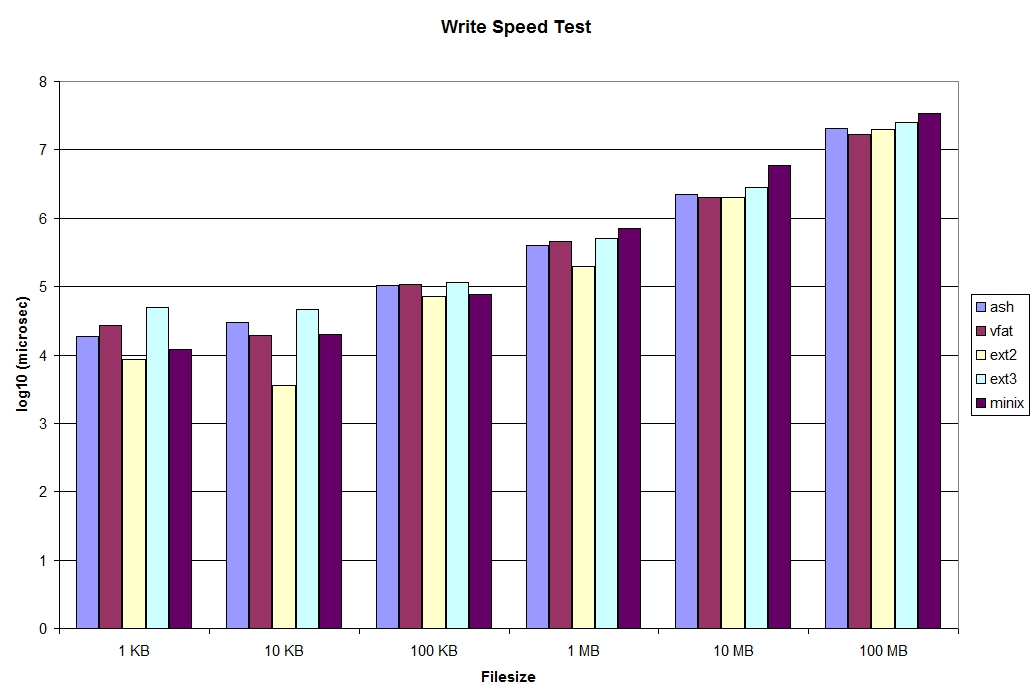
\includegraphics[width=3.5in]{writetest.jpg}
\caption{Write Speed Test}
\label{fig_wspeed}
\end{figure}

\begin{figure}[!t]
\centering
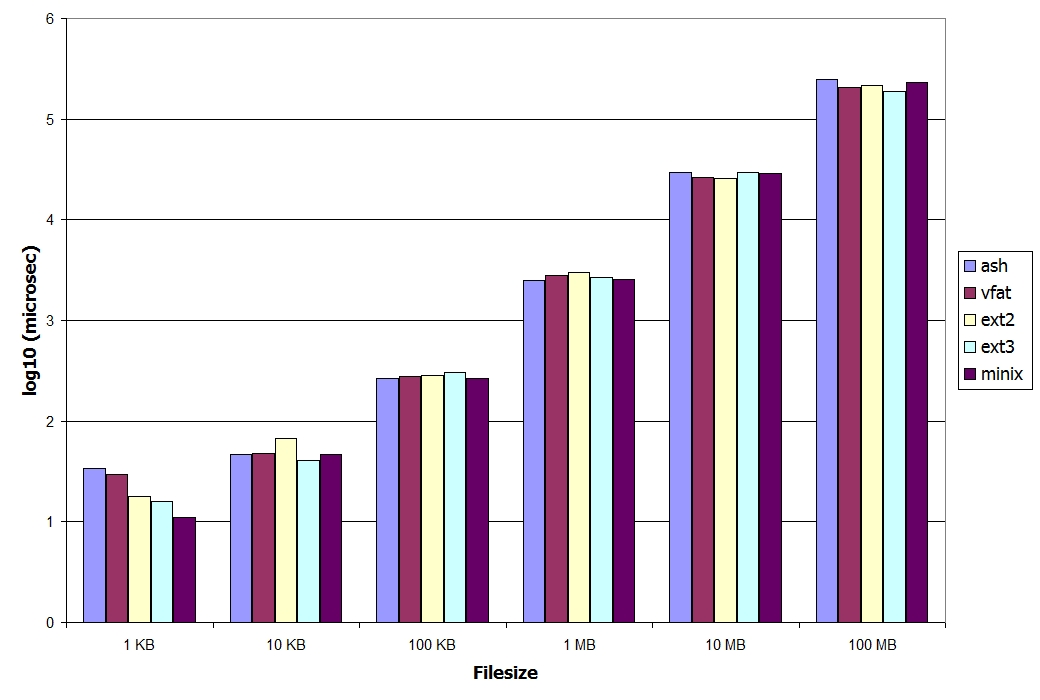
\includegraphics[width=3.5in]{readtest.jpg}
\caption{Read Speed Test}
\label{fig_rspeed}
\end{figure}

\begin{figure}[!t]
\centering
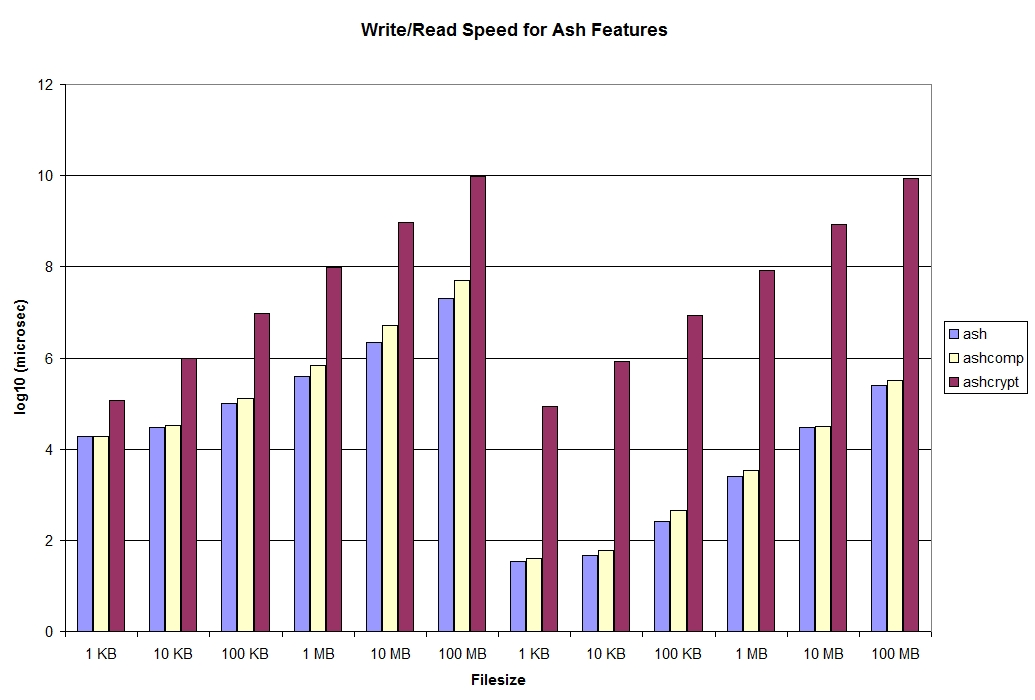
\includegraphics[width=3.5in]{features.jpg}
\caption{Crypting and Compression Speed Test}
\label{fig_fspeed}
\end{figure}


\subsection{Performance tests}
For our comparison tests we use 4 other file systems: {\em vfat}, {\em ext2}, {\em ext3}, {\em minix}. We test write speed, 
read speed, compression speed and encryption speed. \\

The tests have been conducted on VMware Workstation 6.5.0 build 118166, running a Debian 2.6.24.19 generic kernel version on a
Windows Vista Business 32 bit, CPU Core 2 Duo T9300 2.5 GHz and 4 GB RAM, having 1 GB mapped by the virtual machine. The drive used
for the file system was a lowcost HP made 1GB pen drive. The reason for choosing to run VMware for tests is because the tests
cannot model any sort of traffic the user might have for a flash drive, therefore we wished to insert as many latencies as possible
and get the worst case scenario.\\

The tests are conducted for exponentially increasing file sizes of test files, from 1 kB to 100 MB, in powers of 10. The reason
for stopping at 100 MB and not going further to test 1GB is that the biggest files a normal user stores on such drives are mainly
DivX encoded movies, which are always trimmed down to files of 700 MB in size, that can be fitted on a CD.\\

Each test suite will create a file of the given size and attempt 100 cycles of writing it, reading all the file content from disk
and erasing it. During each of the cycles, we measure the speed of the write operation, the read operation and at the end we
obtain the average time in microseconds.\\

Due to the fact that the results increase exponentially along with the file size, the charts used to present them are done in 
logarithmic scale for the time, using the base 10 logarithm.


\section{Future Work}



\subsection{Combine compression with encryption}
In the current version both compression and encryption are supported but separately. At any time you can have 
enabled either compression or encryption but not both at the same time. We must analyse the possibility of 
integrating compression with encryption and see the possible benefits. At a first glance there is one question arising - which of them should be 
done first. 
\subsection{eXecute In Place}
One very nice and useful feature would be {\em eXecute In Place} (XIP) which assumes that the code is
directly executed from the flash drive. When a program residing on {\em AshFS} is run, the executable
code is copied from flash into RAM before the CPU can execute it. Even when the {\em mmap()} system 
call is used, data are not accessed directly from the flash, but are copied into RAM. \\

It is clear that XIP and compression are mutually exclusive: if data are compressed they cannot be 
used directly in place. It is interesting to see then what is the optimal solution: saving an amount of RAM by using
XIP or saving an amount of flash space by using compression. By choosing the latter option, the cost for saving will generally 
be greater than for the former option, because flash is more expensive than RAM. The operating system is more 
flexible in its use of the available RAM, discarding file buffers during the periods of high memory pressure.
Furthermore, because write operations to flash chips are slower, compressing the data is faster in most 
cases.\\

The main problem with XIP is the interaction with the memory management software. Firstly, for all known memory 
management units, each page of data must be page-aligned on the flash in order for it to be mapped into 
processes address space, which makes such a filesystem to waste space. Secondly, while giving write or erase 
commands to a flash chip, it may return status words on all read cycles, therefore all currently valid mappings
would have to be found and invalidated for the duration of operation.

\subsection{Fault Tolerance Support}
We can integrate a 32-bit CRC in every block of data, but this only gives error detection - it does not
allow the filesystem to correct errors. We need more sophisticated methods of dealing with single-bit errors
in flash chips. Possible solutions are using Hamming code, BCH Code or low-density parity-check codes.\\

We can use redundancy to improve fault tolerance. Every critical and high used portion of data must have 
a back up storage. This, of course, will decrease the storage capacity but it can be very useful in 
case of forced unplugging or system crashes.

\subsection{Use linux kernel CryptoAPI}
In the current version we have used a custom implementation of the encryption functions. The linux kernel provides	 
an extensible way of using cryptography by the means of {\em CryptoAPI}. The {\em Scatterlist Crypto API}
takes page vectors (scatterlist) as arguments and works directly on pages. In some cases, this will allow for 
pages to be encrypted in-place with no copying. \\

At the lowest level are the algorithms which register dynamically with the API. Transforms are user-instantiated 
objects, which maintain state, handle all of the implementation logic, manipulate page vectors and 
provide an abstraction to the underlying algorithms.

\subsection{Transaction Support}
For storing database information in AshFS filesystem, it may be desirable to expose transactions 
to userspace. Of course, the userspace can implement transactions itself, using only the file system 
functionality required by POSIX but implementing a transaction-based system on top of AshFS would 
be far less efficient than using the internal functions of the filesystem.

\section{Conclusions}
Our tests have revealed that Linux VFS offers a framework that supports costly operations such as
crypting and compression to be implemented as an intermediate layer in a filesystem without
affecting performance to a very large scale.\\

Across different filesystem implementations, the speed test for the Read operation yielded uniform results.
The difference between implementations is more important for the Write operation, where timings differ to a greater
extent. Writing timings grow in a liniar way in respect to the file size, because flash drives have constant lookup
latency and zero spin time.\\ 

Using an official library for the crypting algorithm instead of a custom tailored implementation will
improve performance considerably. Symmetric crypting algorithms are also the fastest algorithms available for the
needed level of security, which can be increased by selecting a proper length for the used key, between 128, 192 and 256
bits variants. The compression algorithms can be chosen from a larger number of available implementations but using more
complex algorithms than zlib will add higher latencies to the Write operation.\\

Overall, the AshFS project demonstrates how compression and crypting can be combined in order to achieve higher
functionality in the operating system. It is also a proof of concept for how a new filesystem can be integrated with
the existing VFS functionality.

%\subsubsection{Subsubsection Heading Here}
%Subsubsection text here.


% An example of a floating figure using the graphicx package.
% Note that \label must occur AFTER (or within) \caption.
% For figures, \caption should occur after the \includegraphics.
% Note that IEEEtran v1.7 and later has special internal code that
% is designed to preserve the operation of \label within \caption
% even when the captionsoff option is in effect. However, because
% of issues like this, it may be the safest practice to put all your
% \label just after \caption rather than within \caption{}.
%
% Reminder: the "draftcls" or "draftclsnofoot", not "draft", class
% option should be used if it is desired that the figures are to be
% displayed while in draft mode.
%
%\begin{figure}[!t]
%\centering
%\includegraphics[width=2.5in]{myfigure}
% where an .eps filename suffix will be assumed under latex, 
% and a .pdf suffix will be assumed for pdflatex; or what has been declared
% via \DeclareGraphicsExtensions.
%\caption{Simulation Results}
%\label{fig_sim}
%\end{figure}

% Note that IEEE typically puts floats only at the top, even when this
% results in a large percentage of a column being occupied by floats.


% An example of a double column floating figure using two subfigures.
% (The subfig.sty package must be loaded for this to work.)
% The subfigure \label commands are set within each subfloat command, the
% \label for the overall figure must come after \caption.
% \hfil must be used as a separator to get equal spacing.
% The subfigure.sty package works much the same way, except \subfigure is
% used instead of \subfloat.
%
%\begin{figure*}[!t]
%\centerline{\subfloat[Case I]\includegraphics[width=2.5in]{subfigcase1}%
%\label{fig_first_case}}
%\hfil
%\subfloat[Case II]{\includegraphics[width=2.5in]{subfigcase2}%
%\label{fig_second_case}}}
%\caption{Simulation results}
%\label{fig_sim}
%\end{figure*}
%
% Note that often IEEE papers with subfigures do not employ subfigure
% captions (using the optional argument to \subfloat), but instead will
% reference/describe all of them (a), (b), etc., within the main caption.


% An example of a floating table. Note that, for IEEE style tables, the 
% \caption command should come BEFORE the table. Table text will default to
% \footnotesize as IEEE normally uses this smaller font for tables.
% The \label must come after \caption as always.
%
%\begin{table}[!t]
%% increase table row spacing, adjust to taste
%\renewcommand{\arraystretch}{1.3}
% if using array.sty, it might be a good idea to tweak the value of
% \extrarowheight as needed to properly center the text within the cells
%\caption{An Example of a Table}
%\label{table_example}
%\centering
%% Some packages, such as MDW tools, offer better commands for making tables
%% than the plain LaTeX2e tabular which is used here.
%\begin{tabular}{|c||c|}
%\hline
%One & Two\\
%\hline
%Three & Four\\
%\hline
%\end{tabular}
%\end{table}


% Note that IEEE does not put floats in the very first column - or typically
% anywhere on the first page for that matter. Also, in-text middle ("here")
% positioning is not used. Most IEEE journals/conferences use top floats
% exclusively. Note that, LaTeX2e, unlike IEEE journals/conferences, places
% footnotes above bottom floats. This can be corrected via the \fnbelowfloat
% command of the stfloats package.



%\section{Conclusion}
%The conclusion goes here.




% conference papers do not normally have an appendix


% use section* for acknowledgement
%\section*{Acknowledgment}


%The authors would like to thank...





% trigger a \newpage just before the given reference
% number - used to balance the columns on the last page
% adjust value as needed - may need to be readjusted if
% the document is modified later
%\IEEEtriggeratref{8}
% The "triggered" command can be changed if desired:
%\IEEEtriggercmd{\enlargethispage{-5in}}

% references section

% can use a bibliography generated by BibTeX as a .bbl file
% BibTeX documentation can be easily obtained at:
% http://www.ctan.org/tex-archive/biblio/bibtex/contrib/doc/
% The IEEEtran BibTeX style support page is at:
% http://www.michaelshell.org/tex/ieeetran/bibtex/
%\bibliographystyle{IEEEtran}
% argument is your BibTeX string definitions and bibliography database(s)
%\bibliography{IEEEabrv,../bib/paper}
%
% <OR> manually copy in the resultant .bbl file
% set second argument of \begin to the number of references
% (used to reserve space for the reference number labels box)
\begin{thebibliography}{1}
\bibitem{IEEhowto:lka}
Wolfgang Mauer, \emph{Proffesional Linux Kernel Architecture},
Wiley Publishing Inc.
\bibitem{IEEhowto:ulk}
Daniel Bovet , \emph{Understanding the Linux Kernel},
O'Reilley Publishing Inc.
\bibitem{IEEhowto:eld}
Sreekrishnan Venkateswaran, \emph{Essential Linux Device Drivers},
Prentice Hall Publishing
\bibitem{IEEEhowto:dwood}
David Woodhouse, \emph{JFFS: The Journaling Flash File System},
Ottawa Linux Symposium,2001

\bibitem{IEEEhowto:kimlee}
Han-Joon Kim, Sang-Goo Lee, \emph{A new flash memory management
for flash storage system}, COMPSAC '99

\bibitem{IEEEhowto:manni}
Charles Manning, \emph{YAFFS: the NAND-specific flash file system},
Linuxdevices.org, September 20th 2002

\bibitem{IEEEhowto:toledo}
Eran Gal, Sivan Toledo, \emph{A Transactional Flash File System for
Microcontrollers}, USENIX '05

\bibitem{IEEEhowto:park}
Seung-Ho Lim, Kyu-Ho Park, \emph{An efficient NAND flash file
system for flash memory storage}, IEEE Transaction on Computers, 55th Vol.,
July 2006

\end{thebibliography}




% that's all folks
\end{document}


